\section{Modified ResNet50 Architecture}

\tikzset{every picture/.style={line width=0.75pt}}
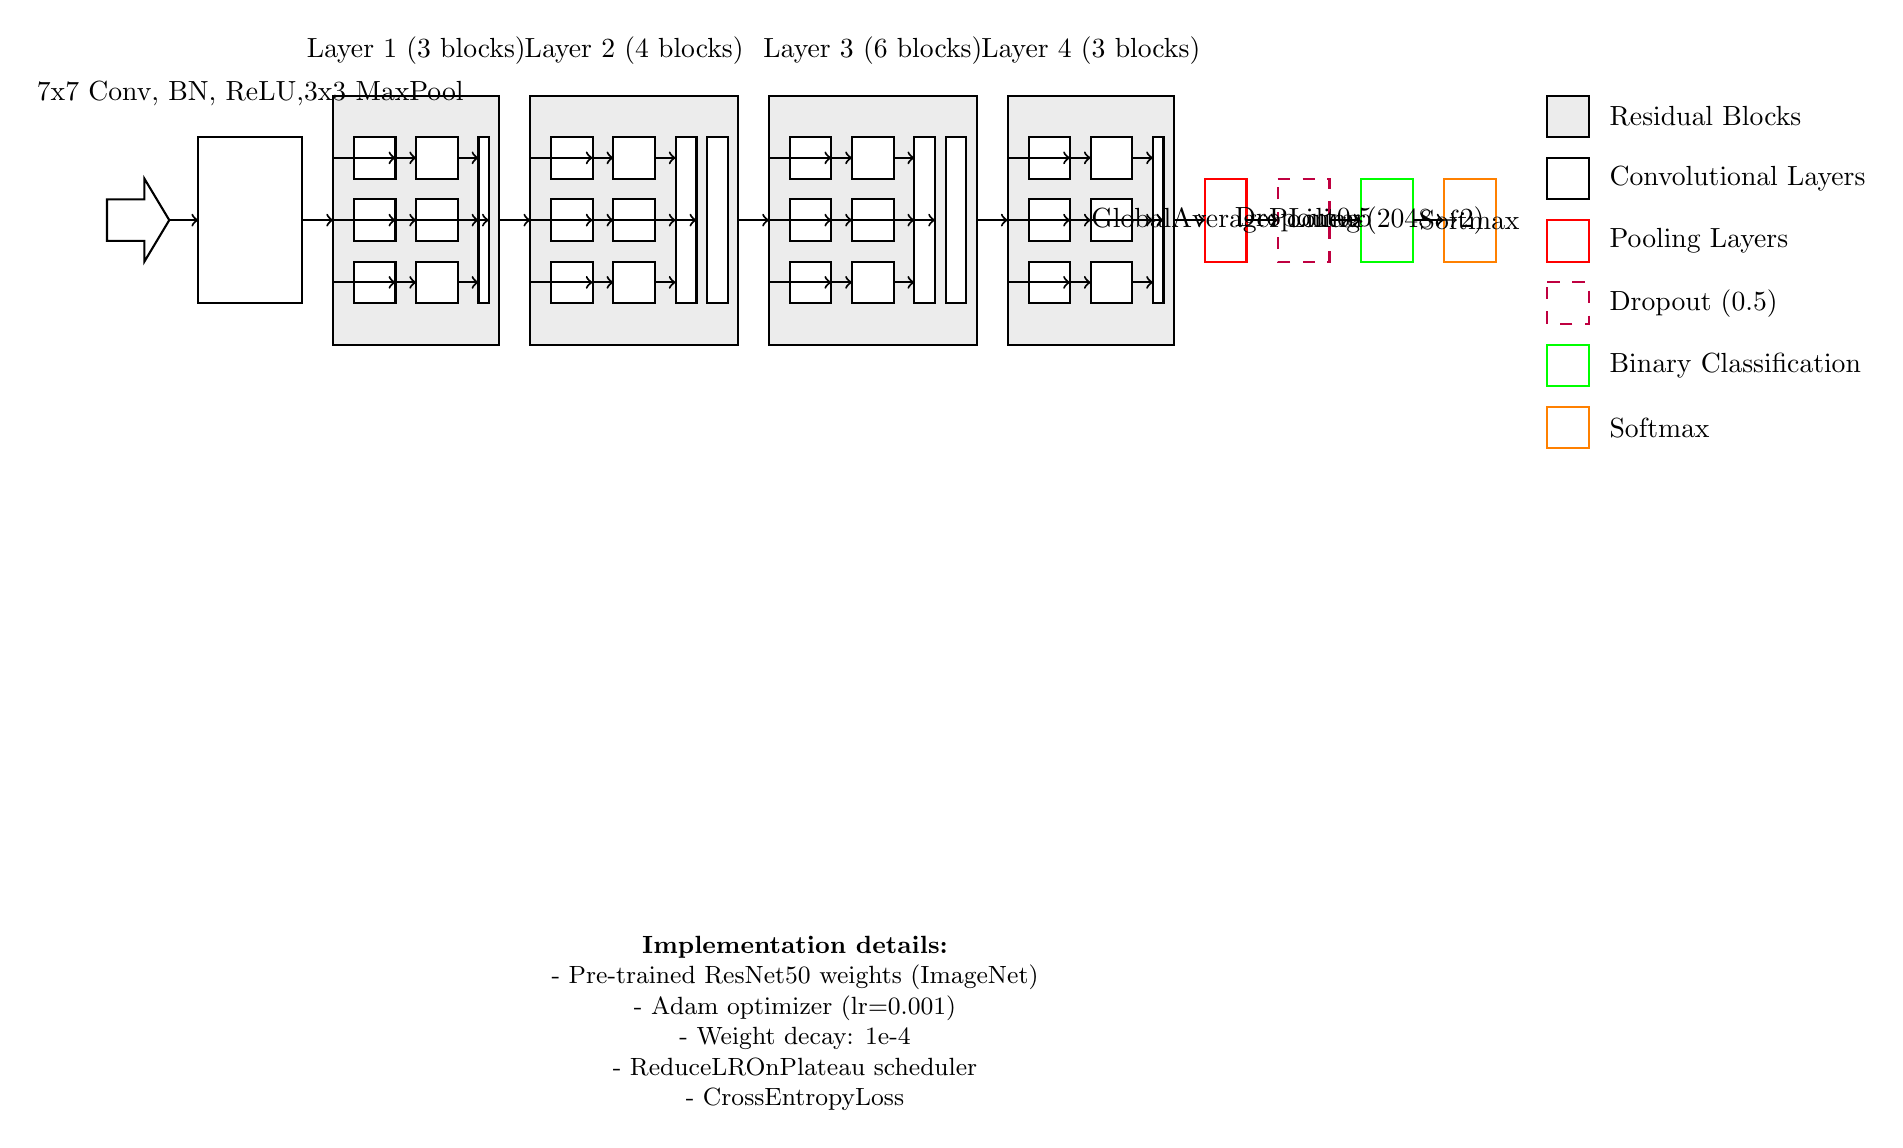
\begin{tikzpicture}[x=0.75pt,y=0.75pt,yscale=-1,xscale=1]

% Input
\draw   (6,150) -- (24,150) -- (24,140) -- (36,160) -- (24,180) -- (24,170) -- (6,170) -- cycle ;

% Stem: Conv + BN + ReLU + MaxPool
\draw  [fill=white  ,fill opacity=1 ] (50,120) -- (100,120) -- (100,200) -- (50,200) -- cycle ;

% Residual Blocks - Layer 1 (3 blocks)
\draw  [fill=lightgray  ,fill opacity=0.3 ] (115,100) -- (195,100) -- (195,220) -- (115,220) -- cycle ;
\draw  [fill=white  ,fill opacity=1 ] (125,120) -- (145,120) -- (145,140) -- (125,140) -- cycle ;
\draw  [fill=white  ,fill opacity=1 ] (125,150) -- (145,150) -- (145,170) -- (125,170) -- cycle ;
\draw  [fill=white  ,fill opacity=1 ] (125,180) -- (145,180) -- (145,200) -- (125,200) -- cycle ;
\draw [->] (125,130) -- (145,130);
\draw [->] (125,160) -- (145,160);
\draw [->] (125,190) -- (145,190);
\draw  [fill=white  ,fill opacity=1 ] (155,120) -- (175,120) -- (175,140) -- (155,140) -- cycle ;
\draw  [fill=white  ,fill opacity=1 ] (155,150) -- (175,150) -- (175,170) -- (155,170) -- cycle ;
\draw  [fill=white  ,fill opacity=1 ] (155,180) -- (175,180) -- (175,200) -- (155,200) -- cycle ;
\draw [->] (145,130) -- (155,130);
\draw [->] (145,160) -- (155,160);
\draw [->] (145,190) -- (155,190);
\draw [->] (175,130) -- (185,130);
\draw [->] (175,160) -- (185,160);
\draw [->] (175,190) -- (185,190);
\draw  [fill=white  ,fill opacity=1 ] (185,120) -- (190,120) -- (190,200) -- (185,200) -- cycle ;
\draw [-] (115,130) -- (125,130);
\draw [-] (115,160) -- (125,160);
\draw [-] (115,190) -- (125,190);
\draw [->] (115,160) -- (190,160);

% Residual Blocks - Layer 2 (4 blocks)
\draw  [fill=lightgray  ,fill opacity=0.3 ] (210,100) -- (310,100) -- (310,220) -- (210,220) -- cycle ;
\draw  [fill=white  ,fill opacity=1 ] (220,120) -- (240,120) -- (240,140) -- (220,140) -- cycle ;
\draw  [fill=white  ,fill opacity=1 ] (220,150) -- (240,150) -- (240,170) -- (220,170) -- cycle ;
\draw  [fill=white  ,fill opacity=1 ] (220,180) -- (240,180) -- (240,200) -- (220,200) -- cycle ;
\draw [->] (220,130) -- (240,130);
\draw [->] (220,160) -- (240,160);
\draw [->] (220,190) -- (240,190);
\draw  [fill=white  ,fill opacity=1 ] (250,120) -- (270,120) -- (270,140) -- (250,140) -- cycle ;
\draw  [fill=white  ,fill opacity=1 ] (250,150) -- (270,150) -- (270,170) -- (250,170) -- cycle ;
\draw  [fill=white  ,fill opacity=1 ] (250,180) -- (270,180) -- (270,200) -- (250,200) -- cycle ;
\draw [->] (240,130) -- (250,130);
\draw [->] (240,160) -- (250,160);
\draw [->] (240,190) -- (250,190);
\draw [->] (270,130) -- (280,130);
\draw [->] (270,160) -- (280,160);
\draw [->] (270,190) -- (280,190);
\draw  [fill=white  ,fill opacity=1 ] (280,120) -- (290,120) -- (290,200) -- (280,200) -- cycle ;
\draw [-] (210,130) -- (220,130);
\draw [-] (210,160) -- (220,160);
\draw [-] (210,190) -- (220,190);
\draw [->] (210,160) -- (290,160);
\draw  [fill=white  ,fill opacity=1 ] (295,120) -- (305,120) -- (305,200) -- (295,200) -- cycle ;

% Residual Blocks - Layer 3 (6 blocks)
\draw  [fill=lightgray  ,fill opacity=0.3 ] (325,100) -- (425,100) -- (425,220) -- (325,220) -- cycle ;
\draw  [fill=white  ,fill opacity=1 ] (335,120) -- (355,120) -- (355,140) -- (335,140) -- cycle ;
\draw  [fill=white  ,fill opacity=1 ] (335,150) -- (355,150) -- (355,170) -- (335,170) -- cycle ;
\draw  [fill=white  ,fill opacity=1 ] (335,180) -- (355,180) -- (355,200) -- (335,200) -- cycle ;
\draw [->] (335,130) -- (355,130);
\draw [->] (335,160) -- (355,160);
\draw [->] (335,190) -- (355,190);
\draw  [fill=white  ,fill opacity=1 ] (365,120) -- (385,120) -- (385,140) -- (365,140) -- cycle ;
\draw  [fill=white  ,fill opacity=1 ] (365,150) -- (385,150) -- (385,170) -- (365,170) -- cycle ;
\draw  [fill=white  ,fill opacity=1 ] (365,180) -- (385,180) -- (385,200) -- (365,200) -- cycle ;
\draw [->] (355,130) -- (365,130);
\draw [->] (355,160) -- (365,160);
\draw [->] (355,190) -- (365,190);
\draw [->] (385,130) -- (395,130);
\draw [->] (385,160) -- (395,160);
\draw [->] (385,190) -- (395,190);
\draw  [fill=white  ,fill opacity=1 ] (395,120) -- (405,120) -- (405,200) -- (395,200) -- cycle ;
\draw [-] (325,130) -- (335,130);
\draw [-] (325,160) -- (335,160);
\draw [-] (325,190) -- (335,190);
\draw [->] (325,160) -- (405,160);
\draw  [fill=white  ,fill opacity=1 ] (410,120) -- (420,120) -- (420,200) -- (410,200) -- cycle ;

% Residual Blocks - Layer 4 (3 blocks)
\draw  [fill=lightgray  ,fill opacity=0.3 ] (440,100) -- (520,100) -- (520,220) -- (440,220) -- cycle ;
\draw  [fill=white  ,fill opacity=1 ] (450,120) -- (470,120) -- (470,140) -- (450,140) -- cycle ;
\draw  [fill=white  ,fill opacity=1 ] (450,150) -- (470,150) -- (470,170) -- (450,170) -- cycle ;
\draw  [fill=white  ,fill opacity=1 ] (450,180) -- (470,180) -- (470,200) -- (450,200) -- cycle ;
\draw [->] (450,130) -- (470,130);
\draw [->] (450,160) -- (470,160);
\draw [->] (450,190) -- (470,190);
\draw  [fill=white  ,fill opacity=1 ] (480,120) -- (500,120) -- (500,140) -- (480,140) -- cycle ;
\draw  [fill=white  ,fill opacity=1 ] (480,150) -- (500,150) -- (500,170) -- (480,170) -- cycle ;
\draw  [fill=white  ,fill opacity=1 ] (480,180) -- (500,180) -- (500,200) -- (480,200) -- cycle ;
\draw [->] (470,130) -- (480,130);
\draw [->] (470,160) -- (480,160);
\draw [->] (470,190) -- (480,190);
\draw [->] (500,130) -- (510,130);
\draw [->] (500,160) -- (510,160);
\draw [->] (500,190) -- (510,190);
\draw  [fill=white  ,fill opacity=1 ] (510,120) -- (515,120) -- (515,200) -- (510,200) -- cycle ;
\draw [-] (440,130) -- (450,130);
\draw [-] (440,160) -- (450,160);
\draw [-] (440,190) -- (450,190);
\draw [->] (440,160) -- (515,160);

% Global Average Pooling
\draw  [color=red  ,draw opacity=1 ][fill=white  ,fill opacity=1 ] (535,140) -- (555,140) -- (555,180) -- (535,180) -- cycle ;

% Dropout Layer
\draw  [color=purple  ,draw opacity=1 ][dash pattern={on 4.5pt off 4.5pt}][fill=white  ,fill opacity=1 ] (570,140) -- (595,140) -- (595,180) -- (570,180) -- cycle ; 

% Binary Classification Layer
\draw  [color=green  ,draw opacity=1 ][fill=white  ,fill opacity=1 ] (610,140) -- (635,140) -- (635,180) -- (610,180) -- cycle ;

% Softmax
\draw  [color=orange  ,draw opacity=1 ][fill=white  ,fill opacity=1 ] (650,140) -- (675,140) -- (675,180) -- (650,180) -- cycle ;

% Connect all components
\draw [->] (36,160) -- (50,160);
\draw [->] (100,160) -- (115,160);
\draw [->] (195,160) -- (210,160);
\draw [->] (310,160) -- (325,160);
\draw [->] (425,160) -- (440,160);
\draw [->] (520,160) -- (535,160);
\draw [->] (555,160) -- (570,160);
\draw [->] (595,160) -- (610,160);
\draw [->] (635,160) -- (650,160);

% Text labels - Adjusted positions
\draw (75,110) node [anchor=south]  {7x7 Conv, BN, ReLU,\\3x3 MaxPool};
\draw (155,90) node [anchor=south]  {Layer 1 (3 blocks)};
\draw (260,90) node [anchor=south]  {Layer 2 (4 blocks)};
\draw (375,90) node [anchor=south]  {Layer 3 (6 blocks)};
\draw (480,90) node [anchor=south]  {Layer 4 (3 blocks)};
\draw (545,160) node [anchor=center]  {Global\\Average\\Pooling};
\draw (582.5,160) node [anchor=center]  {Dropout\\0.5};
\draw (622.5,160) node [anchor=center]  {Linear\\(2048→2)};
\draw (662.5,160) node [anchor=center]  {Softmax};

% Legend - Moved further right and down
\draw  [fill=lightgray  ,fill opacity=0.3 ] (700,100) -- (720,100) -- (720,120) -- (700,120) -- cycle ;
\draw  [fill=white  ,fill opacity=1 ] (700,130) -- (720,130) -- (720,150) -- (700,150) -- cycle ;
\draw  [color=red  ,draw opacity=1 ][fill=white  ,fill opacity=1 ] (700,160) -- (720,160) -- (720,180) -- (700,180) -- cycle ;
\draw  [color=purple  ,draw opacity=1 ][dash pattern={on 4.5pt off 4.5pt}][fill=white  ,fill opacity=1 ] (700,190) -- (720,190) -- (720,210) -- (700,210) -- cycle ;
\draw  [color=green  ,draw opacity=1 ][fill=white  ,fill opacity=1 ] (700,220) -- (720,220) -- (720,240) -- (700,240) -- cycle ;
\draw  [color=orange  ,draw opacity=1 ][fill=white  ,fill opacity=1 ] (700,250) -- (720,250) -- (720,270) -- (700,270) -- cycle ;

\draw (725,110) node [anchor=west]  {Residual Blocks};
\draw (725,140) node [anchor=west]  {Convolutional Layers};
\draw (725,170) node [anchor=west]  {Pooling Layers};
\draw (725,200) node [anchor=west]  {Dropout (0.5)};
\draw (725,230) node [anchor=west]  {Binary Classification};
\draw (725,260) node [anchor=west]  {Softmax};

% Implementation details - Moved further down and centered
\draw (337.5,500) node [anchor=north] [align=center] [font=\small] {\textbf{Implementation details:}\\
- Pre-trained ResNet50 weights (ImageNet)\\
- Adam optimizer (lr=0.001)\\
- Weight decay: 1e-4\\
- ReduceLROnPlateau scheduler\\
- CrossEntropyLoss};

\end{tikzpicture} 